\titledquestion{Understanding word2vec}[20]
Recall that the key insight behind {\tt word2vec} is that \textit{`a word is known by the company it keeps'}. Concretely, consider a `center' word $c$ surrounded before and after by a context of a certain length. We term words in this contextual window `outside words' ($O$). For example, in Figure~\ref{fig:word2vec}, the context window length is 2, the center word $c$ is `banking', and the outside words are `turning', `into', `crises', and `as':

\begin{figure}[h]
    \centering
    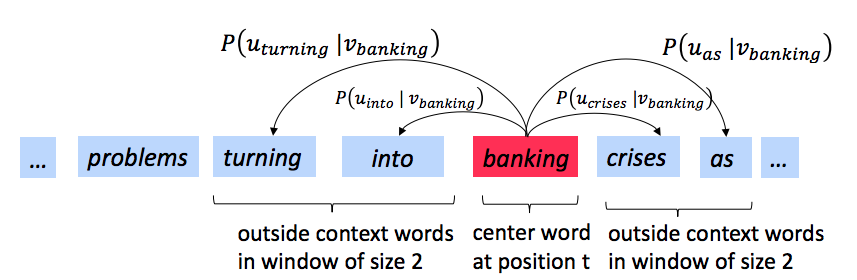
\includegraphics[width=0.6\textwidth]{word2vec.png}
    \caption{The word2vec skip-gram prediction model with window size 2}
    \label{fig:word2vec}
\end{figure}

Skip-gram {\tt word2vec} aims to learn the probability distribution $P(O|C)$. 
Specifically, given a specific word $o$ and a specific word $c$, we want to predict $P(O=o|C=c)$: the probability that word $o$ is an `outside' word for $c$ (i.e., that it falls within the contextual window of $c$).
We model this probability by taking the softmax function over a series of vector dot-products:

\begin{equation}
 P(O=o \mid C=c) = \frac{\exp(\bu_{o}^\top \bv_c)}{\sum_{w \in \text{Vocab}} \exp(\bu_{w}^\top \bv_c)}
 \label{word2vec_condprob}
\end{equation}

For each word, we learn vectors $u$ and $v$, where $\bu_o$ is the `outside' vector representing outside word $o$, and $\bv_c$ is the `center' vector representing center word $c$. 
We store these parameters in two matrices, $\bU$ and $\bV$.
The columns of $\bU$ are all the `outside' vectors $\bu_{w}$;
the columns of $\bV$ are all of the `center' vectors $\bv_{w}$. 
Both $\bU$ and $\bV$ contain a vector for every $w \in \text{Vocabulary}$.\footnote{Assume that every word in our vocabulary is matched to an integer number $k$. Bolded lowercase letters represent vectors. $\bu_{k}$ is both the $k^{th}$ column of $\bU$ and the `outside' word vector for the word indexed by $k$. $\bv_k$ is both the $k^{th}$ column of $\bV$ and the `center' word vector for the word indexed by $k$. \textbf{In order to simplify notation we shall interchangeably use $k$ to refer to word $k$ and the index of word $k$.}}\newline

Recall from lectures that, for a single pair of words $c$ and $o$, the loss is given by:

\begin{equation} 
\bJ_{\text{naive-softmax}}(\bv_c, o, \bU) = -\log P(O=o| C=c).
\label{naive-softmax}
\end{equation}

We can view this loss as the cross-entropy\footnote{The \textbf{cross-entropy loss} between the true (discrete) probability distribution $p$ and another distribution $q$ is $-\sum_i p_i \log(q_i)$.} between the true distribution $\by$ and the predicted distribution $\hat{\by}$, for a particular center word c and a particular outside word o. 
Here, both $\by$ and $\hat{\by}$ are vectors with length equal to the number of words in the vocabulary.
Furthermore, the $k^{th}$ entry in these vectors indicates the conditional probability of the $k^{th}$ word being an `outside word' for the given $c$. 
The true empirical distribution $\by$ is a one-hot vector with a 1 for the true outside word $o$, and 0 everywhere else, for this particular example of center word c and outside word o.\footnote{Note that the true conditional probability distribution of context words for the entire training dataset would not be one-hot.}
The predicted distribution $\hat{\by}$ is the probability distribution $P(O|C=c)$ given by our model in equation (\ref{word2vec_condprob}). \newline

\textbf{Note:} Throughout this homework, when computing derivatives, please use the method reviewed during the lecture (i.e. no Taylor Series Approximations).

\begin{parts}
\part[2]
Prove that the naive-softmax loss (Equation \ref{naive-softmax}) is the same as the cross-entropy loss between $\by$  and $\hat{\by}$, i.e. (note that $\by$ 
 (true distribution), $\hat{\by}$ (predicted distribution) are vectors and $\hat{\by}_o$ is a scalar):

\begin{equation} 
-\sum_{w \in \text{Vocab}} \by_w \log(\hat{\by}_w) = - \log (\hat{\by}_o).
\end{equation}

Your answer should be one line. You may describe your answer in words.

\ifans{Since $\mathbf{y}$ is a one-hot vector where $\mathbf{y}_o = 1$ and $\mathbf{y}_w = 0$ for all $w \neq o$, the summation $\sum_{w \in \text{Vocab}} \mathbf{y}_w \log(\hat{\mathbf{y}}_w)$ collapses to only the term where $w = o$, which is $1 \cdot \log(\hat{\mathbf{y}}_o)$. Thus, the equality holds.}

% Question 1-B
\part[6]
\begin{enumerate}[label=\roman*.]
    \item 
    Compute the partial derivative of $\bJ_{\text{naive-softmax}}(\bv_c, o, \bU)$ with respect to $\bv_c$. \emph{Please write your answer in terms of $\by$, $\hat{\by}$, $\bU$, and show your work to receive full credit}.
    
    \ifans{

        Substituting Equation \ref{word2vec_condprob} into Equation \ref{naive-softmax}:
        \begin{align*}
            J &= -\log \left( \frac{\exp(\mathbf{u}_o^\top \mathbf{v}_c)}{\sum_{w \in \text{Vocab}} \exp(\mathbf{u}_w^\top \mathbf{v}_c)} \right) \\
            &= -\mathbf{u}_o^\top \mathbf{v}_c + \log \left( \sum_{w \in \text{Vocab}} \exp(\mathbf{u}_w^\top \mathbf{v}_c) \right)
        \end{align*}
        Taking the partial derivative with respect to $\mathbf{v}_c$:
        \begin{align*}
            \frac{\partial J}{\partial \mathbf{v}_c} &= \frac{\partial}{\partial \mathbf{v}_c} \left( -\mathbf{u}_o^\top \mathbf{v}_c \right) + \frac{\partial}{\partial \mathbf{v}_c} \log \left( \sum_{w \in \text{Vocab}} \exp(\mathbf{u}_w^\top \mathbf{v}_c) \right) \\
            &= -\mathbf{u}_o + \frac{1}{\sum_{w \in \text{Vocab}} \exp(\mathbf{u}_w^\top \mathbf{v}_c)} \cdot \frac{\partial}{\partial \mathbf{v}_c} \left( \sum_{w \in \text{Vocab}} \exp(\mathbf{u}_w^\top \mathbf{v}_c) \right) \\
            &= -\mathbf{u}_o + \frac{\sum_{w \in \text{Vocab}} \exp(\mathbf{u}_w^\top \mathbf{v}_c) \mathbf{u}_w}{\sum_{w \in \text{Vocab}} \exp(\mathbf{u}_w^\top \mathbf{v}_c)} \\
            &= -\mathbf{u}_o + \sum_{w \in \text{Vocab}} \left( \frac{\exp(\mathbf{u}_w^\top \mathbf{v}_c)}{\sum_{k \in \text{Vocab}} \exp(\mathbf{u}_k^\top \mathbf{v}_c)} \right) \mathbf{u}_w \\
            &= -\mathbf{u}_o + \sum_{w \in \text{Vocab}} \hat{\mathbf{y}}_w \mathbf{u}_w
        \end{align*}
        Using vectorized notation where $\mathbf{u}_o = \mathbf{U}\mathbf{y}$ and $\sum_{w} \hat{\mathbf{y}}_w \mathbf{u}_w = \mathbf{U}\hat{\mathbf{y}}$:
        $$\frac{\partial J}{\partial \mathbf{v}_c} = \mathbf{U}(\hat{\mathbf{y}} - \mathbf{y})$$
    }
    \begin{itemize} 
        \item \textbf{Note}: Your final answers for the partial derivative should follow the shape convention: the partial derivative of any function $f(x)$ with respect to $x$ should have the \textbf{same shape} as $x$.\footnote{This allows us to efficiently minimize a function using gradient descent without worrying about reshaping or dimension mismatching. While following the shape convention, we're guaranteed that $\theta:= \theta - \alpha\frac{\partial J(\theta)}{\partial \theta}$ is a well-defined update rule.}
        \item Please provide your answers for the partial derivative in vectorized form. For example, when we ask you to write your answers in terms of $\by$, $\hat{\by}$, and $\bU$, you may not refer to specific elements of these terms in your final answer (such as $\by_1$, $\by_2$, $\dots$). You may also not refer to specific vectors such as $u_0$, $u_1$, etc.
    \end{itemize}
    \item
    When is the gradient you computed equal to zero? Write a mathematical equation. \\
    \textbf{Hint:} You may wish to review and use some introductory linear algebra concepts.

    \ifans{

        The gradient is zero when $\hat{\mathbf{y}} = \mathbf{y}$. 
        
        Since $\hat{\mathbf{y}}$ is the predicted probability distribution and $\mathbf{y}$ is the ground-truth one-hot vector, this equality holds when the model's prediction is perfect, i.e., $P(O=o|C=c) = 1$ and $P(O=w|C=c) = 0$ for all $w \neq o$.
    }
    \item
    The gradient you found is the difference between the two terms. Provide an interpretation of how each of these terms improves the word vector when this gradient is subtracted from the word vector $v_c$.
    
    \ifans{

        The update rule for gradient descent is $\mathbf{v}_c \leftarrow \mathbf{v}_c - \eta \frac{\partial J}{\partial \mathbf{v}_c}$. Substituting our result:
        $$\mathbf{v}_c \leftarrow \mathbf{v}_c + \eta (\mathbf{u}_o - \sum_{w \in \text{Vocab}} \hat{\mathbf{y}}_w \mathbf{u}_w)$$
        The interpretation of the two terms is as follows:
        \begin{enumerate}
            \item \textbf{The observed term $\mathbf{u}_o$}: Since the similarity between words is measured by their dot product, adding a fraction of $\mathbf{u}_o$ to $\mathbf{v}_c$ reduces the angle between these two vectors. This increases their dot product and makes $\mathbf{v}_c$ more similar to the actual outside word vector, thereby increasing the probability of the true context word.
            \item \textbf{The expectation term $\sum_{w} \hat{\mathbf{y}}_w \mathbf{u}_w$}: This term represents the "average" context word vector as predicted by the current model. By subtracting this from $\mathbf{v}_c$, we move $\mathbf{v}_c$ away from words that the model incorrectly assigns high probability to, effectively "de-biasing" the prediction.
        \end{enumerate}
    }
\end{enumerate}



% Question 1-C
\part[1]
In many downstream applications using word embeddings, L2 normalized vectors (e.g. $\mathbf{u}/||\mathbf{u}||_2$ where $||\mathbf{u}||_2 = \sqrt{\sum_i u_i^2}$) are used instead of their raw forms (e.g. $\mathbf{u}$). Let’s consider a hypothetical downstream task of binary classification of phrases as being positive or negative, where you decide the sign based on the sum of individual embeddings of the words. When would L2 normalization take away useful information for the downstream task? When would it not?

\textbf{Hint:} Consider the case where $\mathbf{u}_x = \alpha\mathbf{u}_y$ for some words $x \neq y$ and some scalar $\alpha$. When $\alpha$ is positive, what will be the value of normalized  $\mathbf{u}_x$ and normalized $\mathbf{u}_y$? How might $\mathbf{u}_x$ and $\mathbf{u}_y$ be related for such a normalization to affect or not affect the resulting classification?

\ifans{

    L2 normalization takes away useful information when the magnitude of the word vector represents its semantic intensity or importance. For example, if $\mathbf{u}_{excellent} = \alpha \mathbf{u}_{good}$ with $\alpha > 1$, normalization would make them identical, losing the information that "excellent" is a stronger positive signal than "good" in a sum of embeddings.
    
    It would not take away useful information (and might even help) if the magnitude mainly reflects word frequency or noise rather than meaning. In such cases, the direction of the vector captures the core semantics, and normalization prevents high-frequency words from disproportionately dominating the classification result.
}

% Question 1-D
\part[1]
Write down the partial derivative of $\bJ_{\text{naive-softmax}}(\bv_c, o, \bU)$ with respect to $\bU$. Please break down your answer in terms of the column vectors $\frac{\partial \bJ(\bv_c, o, \bU)}{\partial \bu_1}$, $\frac{\partial \bJ(\bv_c, o, \bU)}{\partial \bu_2}$, $\cdots$, $\frac{\partial \bJ(\bv_c, o, \bU)}{\partial \bu_{|\text{Vocab}|}}$ (do not further expand these terms). No derivations are necessary, just an answer in the form of a matrix.

\ifans{
    $$\frac{\partial J}{\partial \mathbf{U}} = \begin{bmatrix} 
    \frac{\partial J}{\partial \mathbf{u}_1} & \frac{\partial J}{\partial \mathbf{u}_2} & \cdots & \frac{\partial J}{\partial \mathbf{u}_{|\text{Vocab}|}}
    \end{bmatrix}$$
}

% Question 1-E
\part[5] 
Compute the partial derivatives of $\bJ_{\text{naive-softmax}}(\bv_c, o, \bU)$ with respect to each of the `outside' word vectors, $\bu_w$'s. There will be two cases: when $w=o$, the true `outside' word vector, and $w \neq o$, for all other words. Please write your answer in terms of $\by$, $\hat{\by}$, and $\bv_c$. In this subpart, you may use specific elements within these terms as well (such as $\by_1$, $\by_2$, $\dots$). Note that $\bu_w$ is a vector while $\by_1, \by_2, \dots$ are scalars. Show your work to receive full credit.

\ifans{

    The loss function is $J = -\mathbf{u}_o^\top \mathbf{v}_c + \log \sum_{k \in \text{Vocab}} \exp(\mathbf{u}_k^\top \mathbf{v}_c)$.
    
    \textbf{Case 1: $w = o$}
    \begin{align*}
        \frac{\partial J}{\partial \mathbf{u}_o} &= \frac{\partial}{\partial \mathbf{u}_o} \left( -\mathbf{u}_o^\top \mathbf{v}_c \right) + \frac{\partial}{\partial \mathbf{u}_o} \log \left( \sum_{k \in \text{Vocab}} \exp(\mathbf{u}_k^\top \mathbf{v}_c) \right) \\
        &= -\mathbf{v}_c + \frac{1}{\sum_{k \in \text{Vocab}} \exp(\mathbf{u}_k^\top \mathbf{v}_c)} \cdot \exp(\mathbf{u}_o^\top \mathbf{v}_c) \mathbf{v}_c \\
        &= -\mathbf{v}_c + \hat{y}_o \mathbf{v}_c = (\hat{y}_o - 1) \mathbf{v}_c
    \end{align*}
    
    \textbf{Case 2: $w \neq o$}
    \begin{align*}
        \frac{\partial J}{\partial \mathbf{u}_w} &= 0 + \frac{\partial}{\partial \mathbf{u}_w} \log \left( \sum_{k \in \text{Vocab}} \exp(\mathbf{u}_k^\top \mathbf{v}_c) \right) \\
        &= \frac{1}{\sum_{k \in \text{Vocab}} \exp(\mathbf{u}_k^\top \mathbf{v}_c)} \cdot \exp(\mathbf{u}_w^\top \mathbf{v}_c) \mathbf{v}_c \\
        &= \hat{y}_w \mathbf{v}_c
    \end{align*}
    
    Since $y_o = 1$ and $y_w = 0$ for $w \neq o$, both cases can be summarized as:
    $$\frac{\partial J}{\partial \mathbf{u}_w} = (\hat{y}_w - y_w) \mathbf{v}_c$$
}
% Question 1-F
\item (2 points) As an additional exercise for this problem, you will be taking the derivatives of some common loss functions, which may be used in variations of {\tt word2vec} (such as the negative sampling variant). The Leaky ReLU (Leaky Rectified Linear Unit) activation function is given by Equation \ref{LeakyReLU} and Figure~\ref{fig:leaky_relu}:
\begin{equation}
    \label{LeakyReLU}
    f(x) = \max(\alpha x, x)
\end{equation}

\begin{figure}[h]
    \centering
    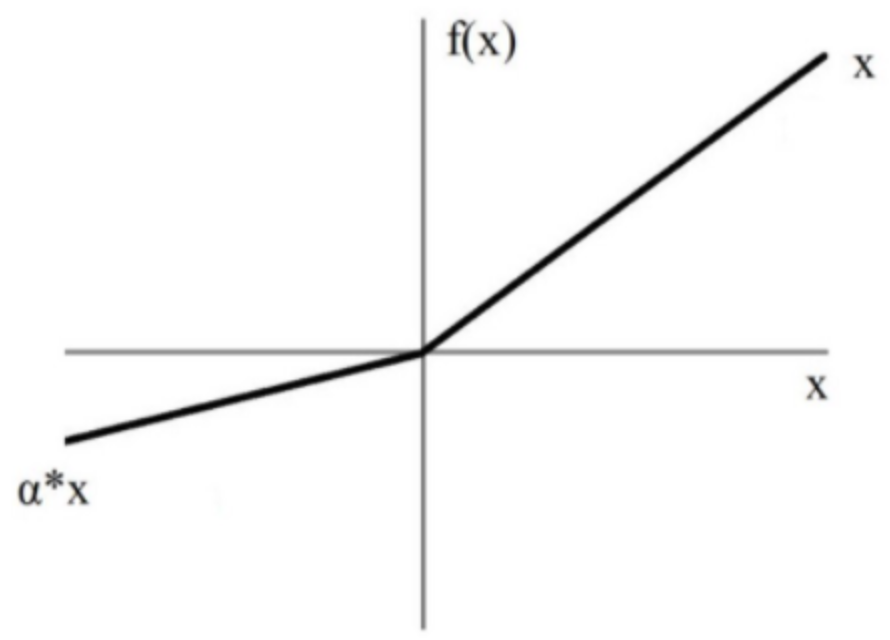
\includegraphics[width=0.3\textwidth]{leaky_relu_graph.png}
    \caption{Leaky ReLU}
    \label{fig:leaky_relu}
\end{figure}

Where $x$ is a scalar and $0<\alpha <1$, please compute the derivative of $f(x)$ with respect to $x$. You may ignore the case where the derivative is not defined at 0.\footnote{If you're interested in how to handle the derivative at this point, you can read more about the notion of \hyperref[https://en.wikipedia.org/wiki/Subderivative]{subderivatives}.}

\ifans{
    For $x \neq 0$, the derivative of $f(x) = \max(\alpha x, x)$ is:
    $$f'(x) = \begin{cases} 
      1 & \text{if } x > 0 \\
      \alpha & \text{if } x < 0 
    \end{cases}$$
}

% Question 1-G
\item (3 points) The sigmoid function is given by Equation \ref{Sigmoid Function}:

\begin{equation}
    \label{Sigmoid Function}
    \sigma (x) = \frac{1}{1 + e^{-x}} = \frac{e^{x}}{e^{x} + 1}
\end{equation}

Please compute the derivative of $\sigma(x)$ with respect to $x$, where $x$ is a scalar. Please write your answer in terms of $\sigma(x)$. Show your work to receive full credit.

\ifans{
    Using the chain rule:
    \begin{align*}
        \sigma'(x) &= \frac{d}{dx} (1 + e^{-x})^{-1} \\
        &= -1 \cdot (1 + e^{-x})^{-2} \cdot \frac{d}{dx}(1 + e^{-x}) \\
        &= -(1 + e^{-x})^{-2} \cdot (-e^{-x}) \\
        &= \frac{e^{-x}}{(1 + e^{-x})^2} \\
        &= \frac{1}{1 + e^{-x}} \cdot \frac{e^{-x}}{1 + e^{-x}} \\
        &= \sigma(x) \cdot \frac{1 + e^{-x} - 1}{1 + e^{-x}} \\
        &= \sigma(x) \cdot (1 - \sigma(x))
    \end{align*}
}

\end{parts}